\documentclass[main]{subfiles}

\begin{document}
\begin{lect}{2019-09-26}
		\begin{Reminder}
				\[(1) \q \dot{x} = X(t, x), \q\q X(t, x) \in C(G) \q \underbracket{G}_{\text{Обл}} \subset \R^2 \]
				\[(2) \q (t_0, x_0) \in G\]
		\end{Reminder}

		\begin{Theorem}
				\[\exists \underbracket{V}_{\text{окр}} (t_0, x_0) \subset G : \q
				\frac{\partial X}{\partial x} \in C(V(t_0, x_0))\]
				\[\Ra (t_0, x_0) \text{ - точка ед-ти}\]
		\end{Theorem}

		\begin{Consequence}
				\[X \in C(G), \q \frac{\partial X}{\partial x} \in C(G) \Ra G \text{ - обл ед-ти}\]
		\end{Consequence}

		\begin{proof}
		    \begin{enumerate}
			    	\item $\exists a>0, b>0:$
						\[D = \{(t, x) : \abs{t - t_0} \leq a,\ \abs{x - x_0} \leq b\} \subset V(t_0, x_0) \subset G\]
						\[\Ra \exists M: \abs{X(t, x)} \leq M \q \forall (t, x) \in D\]
						\[\exists L : \abs{\frac{\partial X}{\partial x}(t, x)} \leq L \q \forall (t, x) \in D\]
						\[h = \min(a, \frac{b}{M})\]
						\[\Ra \exists \text{Реш}(1),(2) \q x = \varphi(t), \q x \in [t_0 - h, t_0 + h]\]
						\[\underline{\Delta = h}\]
						\[\letus x = \psi(t) \text{ - реш}(1)2(0\]
						\[\text{Докажем: оно определено на } [t_0 - h, t_0 + h] \text{ т.е}\]
						\[\abs{\psi(t) - x_0} \leq b \q \forall t : \abs{t - t_0} \leq h\]
						\[\text{от прот. } \letus \exists t^*: \begin{cases}
							\abs{t^{*} - t_0}  \leq h\\
							\abs{\psi(t^*) - x_0} > b
						\end{cases}\]
						\[t^* \neq t_0 \q (\psi(t_0) = x_0) \q \text{НУО } t^* > t_0 \]
						\[v(t) = \abs{\psi(t) - x_0} - b \text{ - непр}\]
						\[\begin{align}
								&v(t_0) = -b < 0\\
								&v(t^*) > 0
							\end{align}
						\ \bigg| \Ra \exists t_1 : t_0 < t_1 < t^* : \q v(t_1) = 0\]
						\[O = \{t \in [t_0, t^*] : v(t) = 0\} \q O \neq \varnothing \q O \text{ - замк. огр}\]
						\[\Ra \exists \min O = t_2 \q(\text{мб } t_1 = t_2)\]
						\[\forall t \in [t_0, t_2) \q v(t) < 0 \q v(t_2) = 0 \q t_0 < t_2 < t^*\]
						\[\Ra \text{ на } [t_0, t_2] \q \abs{\psi(t) - x_0} \leq b\]
						\[\dot{\psi}(t) = X(t, \psi(t)), \q \psi(t_0) = x_0\]
						\[\text{инт на } [t_0, t_2]\]
						\[\abs{\psi(t_2) - x_0} = \abs{\int_{t_0}^{t_2} X(t, \psi(t))dt} \leq
						\int_{t_0}^{t_2} \abs{\underbracket{X(t, \psi(t))}_{\leq M} }dt  \]
						\[\leq M \cdot (t_2 - t_0) < M(t^* - t_0) \leq Mh \leq b\]
						\[\text{Получим } \abs{\psi(t_2) - x_0} < b \text{ - противореч: } t_2 \in O\]
					\item $t \in [t_0 - h, t_0 + h]$
						\begin{figure}[H]
						    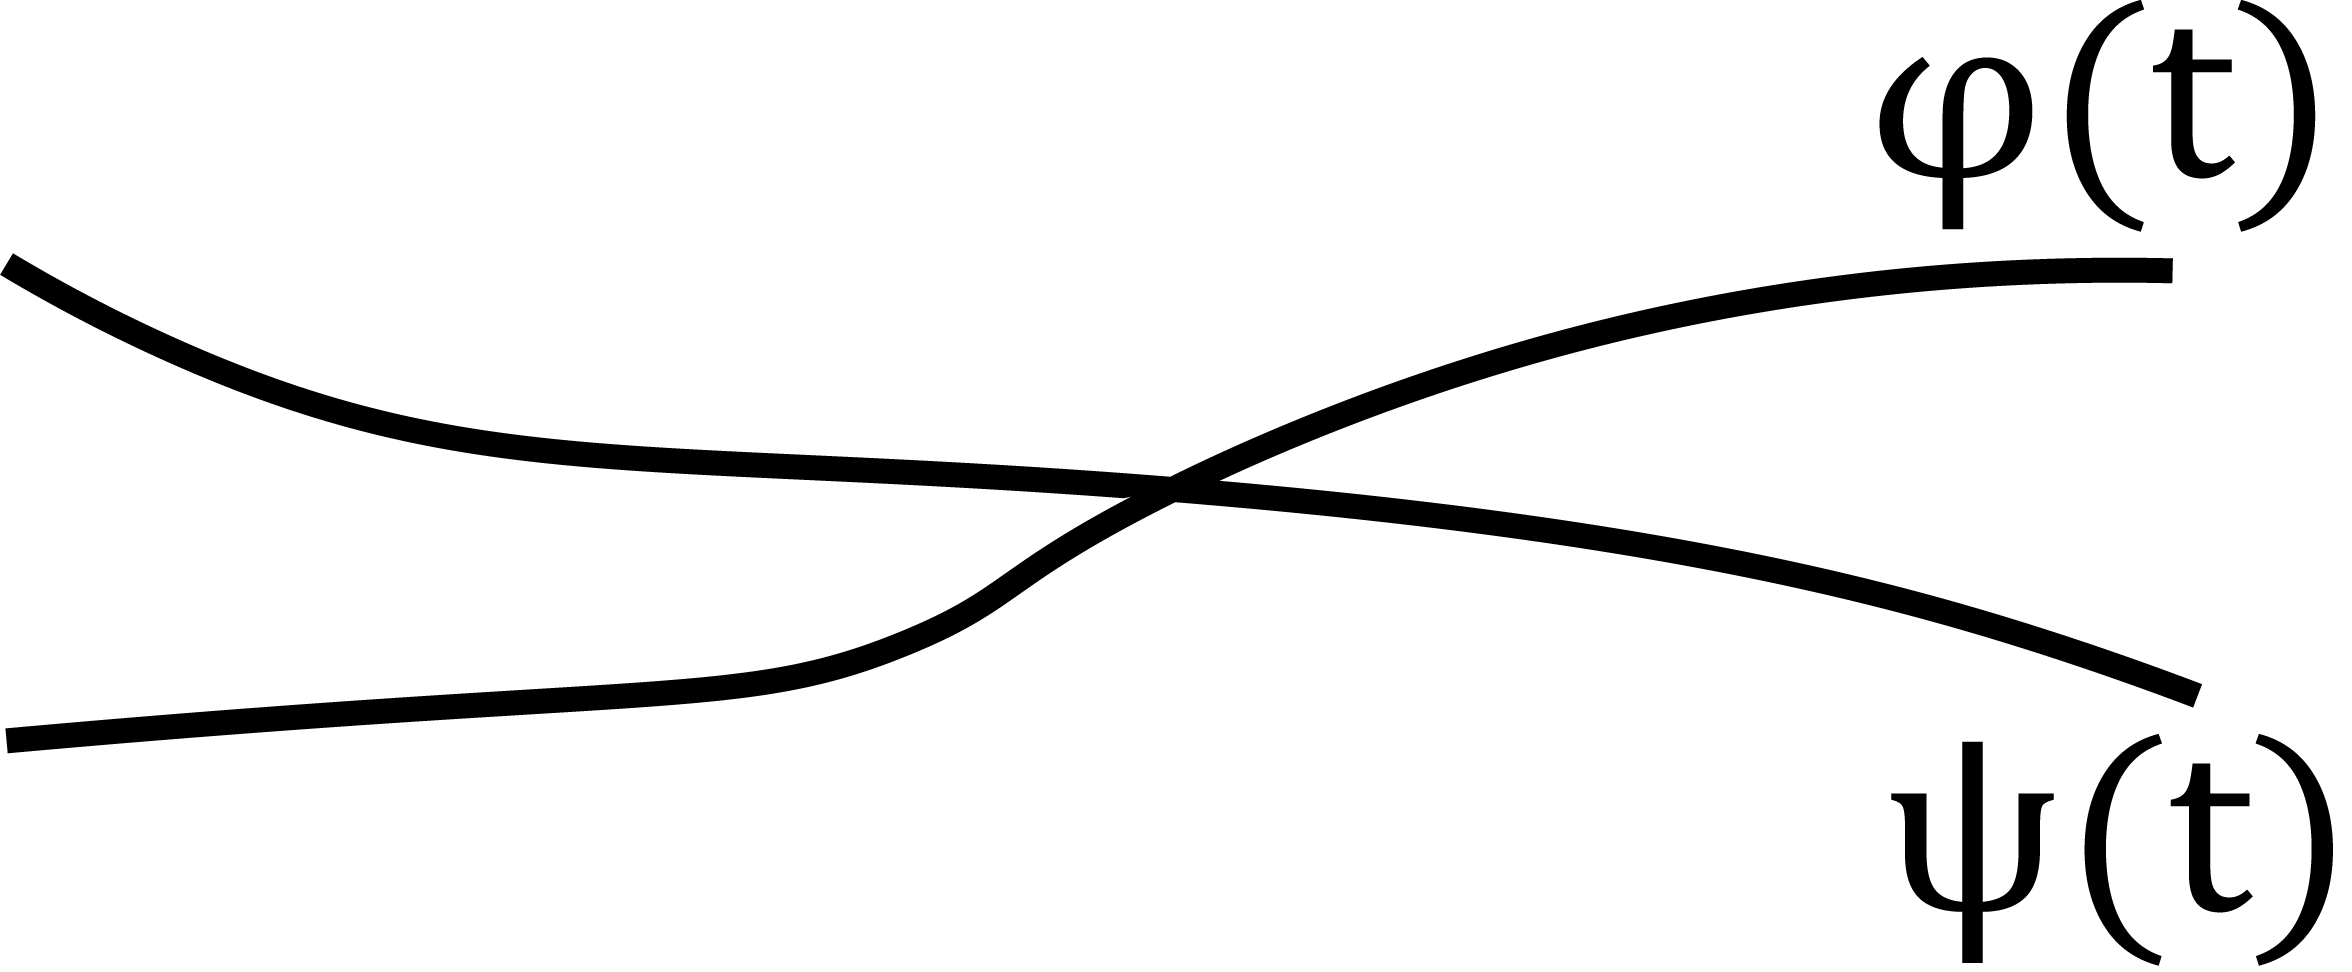
\includegraphics[width=4cm]{pics/4_1.png}
						    \centering
						\end{figure}
						\[f(s) = X(t, s\varphi(t) + (1 - S)\varphi(t)), \q s \in [0, 1]\]
						\[\abs{s \varphi(t) + (1 - s)\psi(t) - x_0} \leq \abs{s \varphi(t) - sx_0} +
						\abs{(1 - s) \psi(t) - (1 - s) x_0 } = \]
						\[= s \abs{ \underbracket{\varphi(t) - x_0}_{\leq b}} + (1-s)
						\abs{\underbracket{\psi(t) - x_0}_{\leq b} } \leq b(s + (1 - s)) = b \Ra\]
						\[\Ra f(s) \text{ опред. при } \abs{t - t_0} \leq h\]
						\[\abs{X(t, \varphi(t)) - X(t, \psi(t))} = \abs{f(1) - f(0)} = \q\q \exists \theta \in (0,1)\]
						\[= \abs{f'(\theta)} = \abs{\frac{\partial X}{\partial x}\Bigg|_{x = s\varphi(t) +
						(1 - s)\psi(t)}  \cdot \frac{\partial x}{\partial s}\Bigg|_{s = \theta}} = \]
						\[= \abs{\underbracket{\frac{\partial X}{\partial x}\Bigg|_{...}}_{\leq L} } \cdot
						\abs{\varphi(t) - \psi(t)}\]
						\[\text{Итог: } \abs{X(t, \varphi(t)) - X(t, \psi(t))} \leq L\abs{\varphi(t) - \psi(t)} \q (5)\]
					\item 	$\dot{\varphi}(t) = X(t, \varphi(t))$
						\[\dot{\psi}(t, \psi(t))\]
						\[\dot{\varphi}(t) - \dot{\psi(t)} = X(t, \varphi(t)) - X(t, \psi(t))\]
						\[\text{Инт. } [t_0, t]\]
						\[\varphi(t) - x_0 - (\psi(t) - x_0) = \int_{t_0}^{t} (X(\tau, \varphi(\tau)) -
						X(\tau, \psi(\tau))) d\tau  \]
						\[\Ra \abs{\varphi(t) - \psi(t)} \leq \abs{\int_{t_0}^t \abs{X(t, \varphi(\tau) -
						X(\tau, \psi(\tau))} d\tau} \leq\]
						\[\leq \cdot\abs{\int_{t_0}^t  \abs{\varphi(t\tau) - \psi(\tau)}d\tau} \os{\text{Л.Г.}}{\Ra}
						\varphi(t) = \psi(t) \q \forall t : \abs{t - t_0} \leq h\]
						\[(u(t) = \abs{\varphi(t) - \psi(t)} : u(t) \leq L \q \abs{\int_{t_0}^t u(\tau) d\tau})\]
				\end{enumerate}
		\end{proof}

		\section{Уравнения в симметричной форме}
		\begin{Definition}
				\[(1) \q M(x, y)dx + N(x, y)dy = 0 \text{ - ур. 1 порядка в симм. форме}\]
				\[M, N \in C(G) \q\q \underbracket{G}_{\text{обл}} \subset \R^2 \]
		\end{Definition}

		\begin{Definition}
				\[\text{ф-я } y = \varphi(x) \q x \in <a, b>\]
				\[(\text{или ф-я } \ x = \psi(y) \q y \in <c, d>)\]
				\[\text{наз. реш. } (1) \text{, если подст в } (1) \text{ получ. тождество}\]
				\[\text{Если } y = \varphi(x) \text{ - реш } (1) \q x \in <a, b>\]
				\[M(x, \varphi(x))dx + N(x, \varphi(x))\varphi'(x)dx = 0\]
				\[y = \varphi(x) \q x \in  <a, b> \text{ - реш.} (1) \rla \]
				\[\rla (2) \q M(x, \varphi(x)) + N(x, \varphi(x)) \varphi'(x) \equiv 0 \text{ на } <a, b>\]
				\[\Ra y = \varphi(x) \text{ удовл. ур-нию } \q\q \text{если } N(x, \varphi(x)) \neq 0 \text{ на } <a, b>\]
				\[(3) \q\q y' = - \frac{M(x, y)}{N(x, y)}\]
				\[\text{аналог: } x = \psi(y) \q y \in <c, d> \text{ - реш }(1) \rla\]
				\[M(\psi(y), y)\psi'(y) + N(\psi(y), y) \equiv 0 \text{ на } <c, d> \q (2')\]
				\[\text{и } x = \psi(y) \text{ уд. ур-нию } \q\q (\text{если } M(\psi(y), y) \neq 0 \text{ на } <c, d>)\]
				\[(3') \q\q x' = - \frac{N(x, y)}{M(x, y)}\]
				\[(x_0, y_0) \in G\]
				\[\text{если } N(x_0, y_0) \neq 0 \Ra \exists <a, b> : x_0 \in (a, b) \q \exists \text{реш }
				y = \varphi(x) \q (3) \text{ (и реш (1))}\]
				\[\text{если } M(x_0, y_0) \neq 0 \Ra \exists <c, d> : y_0 \in (c, d) \q \exists \text{реш }
				x = \psi(y) \q (3') \text{ (и реш (1))}\]
				\[\text{если } M(x_0, y_0) = N(x_0, y_0) = 0 \Ra (x_0, y_0) \text{ - особая точка}\]
		\end{Definition}

		\begin{remark}
				Если $\varphi(x) \text{ - реш}, то \varphi(x)^-1 =$
		\end{remark}

		\begin{Definition}
				\[u(x, y) \in C^{1} \q(u : G \in \R) \text{ интеграл (1), если}\]
				\[1) \q \bigg(\frac{\partial u}{\partial x}\bigg)^2 + \bigg(\frac{\partial u}{\partial y}\bigg)^2
				\neq 0 \q \forall \text{ обык. точки из }G \q (x, y)\]
				\[2) \q (4) \ra N(x, y) \frac{\partial u(x, y)}{\partial x} -
				M(x, y) \frac{\partial u(x, y)}{\partial y} \equiv 0 \text{ в } G\]
				\[(N \frac{\partial u}{\partial x} - M \frac{\partial u}{\partial y} \equiv 0)\]
		\end{Definition}

		\begin{Theorem}[1]
				\[y = \varphi(x) \text{ - реш.(1)} \q x \in <a, b>\]
				\[(x, \varphi(x)) \text{ - обыкн. точка для } \forall x \in <a, b>\]
				\[u(x, y) \text{ - интеграл (1) в } G\]
				\[\Ra u(x, \varphi(x)) = const \q x \in <a, b>\]
		\end{Theorem}

		\begin{Proof}
				\[y = \varphi(x) \text{ - реш (1)} \q x \in <a, b> \Ra\]
				\[\Ra \varphi'(x) = - \frac{M(x, \varphi(x))}{M(x, \varphi(x))} \q\q N(x, \varphi(x)) \neq 0\]
				\[(\text{если N(...) = 0, то } \os{(2)}{\Ra} M(...) = 0 \text{ - против. усл})\]
				\[\frac{d}{dx} u (x, \varphi(x)) = \frac{\partial u(...)}{\partial x} + \frac{\partial u(...)}
				{\partial y} \cdot \varphi'(x) = \]
				\[= \frac{\partial u(...)}{\partial x} + \frac{\partial u(...)}{\partial y}
				(- \frac{M(...)}{N(...)}) = \frac{1}{N(...)} (N(...) \frac{\partial u(...)}{\partial x} -
				M(...) \frac{\partial u(...)}{\partial y})\]
		\end{Proof}

		\begin{Theorem} [1']
				\[x = \psi(y) \text{ - реш }(1) \q y \in <c, d>...\]
		\end{Theorem}
\end{lect}
\end{document}
